\documentclass{article}

% If you're new to LaTeX, here's some short tutorials:
% https://www.overleaf.com/learn/latex/Learn_LaTeX_in_30_minutes
% https://en.wikibooks.org/wiki/LaTeX/Basics

% Formatting
\usepackage[utf8]{inputenc}
\usepackage[margin=1in]{geometry}
\usepackage[titletoc,title]{appendix}

% Math
% https://www.overleaf.com/learn/latex/Mathematical_expressions
% https://en.wikibooks.org/wiki/LaTeX/Mathematics
\usepackage{amsmath,amsfonts,amssymb,mathtools}

% Images
% https://www.overleaf.com/learn/latex/Inserting_Images
% https://en.wikibooks.org/wiki/LaTeX/Floats,_Figures_and_Captions
\usepackage{graphicx,float}

% Tables
% https://www.overleaf.com/learn/latex/Tables
% https://en.wikibooks.org/wiki/LaTeX/Tables

% Algorithms
% https://www.overleaf.com/learn/latex/algorithms
% https://en.wikibooks.org/wiki/LaTeX/Algorithms
\usepackage[ruled,vlined]{algorithm2e}
\usepackage{algorithmic}

% Code syntax highlighting
% https://www.overleaf.com/learn/latex/Code_Highlighting_with_minted
\usepackage{minted}
\usemintedstyle{borland}

% References
% https://www.overleaf.com/learn/latex/Bibliography_management_in_LaTeX
% https://en.wikibooks.org/wiki/LaTeX/Bibliography_Management
\usepackage{biblatex}
\addbibresource{references.bib}

\DeclareMathOperator{\taninv}{tan\,inverse}

% Title content
\title{ENPM 673 Homework 1}
\author{Arjun Srinivasan Ambalam,Praveen Menaka Sekar,Arun Kumar Dhandayuthabani}
\newline
\date{February 05, 2020}

\begin{document}

\maketitle




% Introduction and Overview
\section{Problem 1}


% Example Subsection
\subsection{Since camera sensor is square shaped and also a single focal length is given,the Field of View (FOV) in Horizontal and Vertical directions are same}
\begin{equation*}
FOV , \phi=\tan ^{-1} \frac{d}{2f}
\end{equation*}
 where d is camera sensor width (d=14 mm)
        , f is focal length (f=15 mm)
\begin{equation*}     
   \phi =\tan ^{ - 1}\frac{14}{2*15}
                    
                   \hspace{6.5cm} \phi =  25.0168.
\end{equation*}


% Example Subsubsection
\subsection{Minimum number of pixels occupying image}
Square shaped object with width 5cm (w) = 50 mm,
Distance of from the camera (D) = 20 m = 20000 mm.
Let size of the object image on camera sensor be 'x' mm
\begin{equation*}
 \frac{x}{2f}=\frac{w}{2D}
 \end{equation*}
\begin{flushleft}
After substitution and solving we get x=0.0375 mm,\\
5 MP resolution for sensor area 14\times14\hspace{.1cm}mm ^2 \\
Therefore for sensor area \hspace{.1cm}0.0375*0.0375, Minimum number of corresponding pixels are 35.87
  
\end{flushleft}

\section{Curve Fitting Methods}
We have discussed about Least Squares ,Total Least Squares and Least Squares with Regularization.From the results we see that             method is best fit for the problem in hand. 

\section{Homography in Computer Vision}
% Algorithm Implementation and Development
\section{Algorithm Implementation and Development}
Add your algorithm implementation and development here. See Algorithm~\ref{alg:example} for how to include an algorithm in your document. This is how to make an \textit{ordered} list:
\begin{enumerate}
    \item Fluffy swallowed a marble.
    \item I took Fluffy to the vet.
    \item They took an ultrasound of Fluffy's intestines.
\end{enumerate}

\begin{algorithm}
\begin{algorithmic}
    \STATE{Import data from \texttt{Testdata.mat}}
    \FOR{$j = 1:20$}
        \STATE{Extract measurement $j$ from \texttt{Undata}}
        \STATE{Do something useful}
    \ENDFOR
    \IF{$i\geq 5$} 
        \STATE{$i\gets i-1$}
    \ELSE
        \IF{$i\leq 3$}
            \STATE{$i\gets i+2$}
        \ENDIF
    \ENDIF 
\end{algorithmic}
\caption{Example Algorithm}
\label{alg:example}
\end{algorithm}

% Computational Results
\section{Computational Results}
Add your computational results here. See Table~\ref{tab:mascots} for how to include a table in your document. See Figure~\ref{fig:dubs} for how to include figures in your document.

\begin{table}
    \centering
    \begin{tabular}{rll}
    & Name & Years \\
    \hline
    1 & Frosty & 1922-1930  \\
    2 & Frosty II & 1930-1936 \\
    3 & Wasky & 1946 \\
    4 & Wasky II & 1947 \\
    5 & Ski & 1954 \\
    6 & Denali & 1958 \\
    7 & King Chinook & 1959-1968\\
    8 & Regent Denali & 1969 \\
    9 & Sundodger Denali & 1981-1992 \\
    10 & King Redoubt & 1992-1998 \\
    11 & Prince Redoubt & 1998 \\
    12 & Spirit & 1999-2008 \\
    13 & Dubs I & 2009-2018 \\
    14 & Dubs II & 2018-Present
    \end{tabular}
    \caption{UW mascots as described in \cite{washington_huskies}.}
    \label{tab:mascots}
\end{table}

% begin{figure}[tb] % t = top, b = bottom, etc.
\begin{figure}
    \centering
    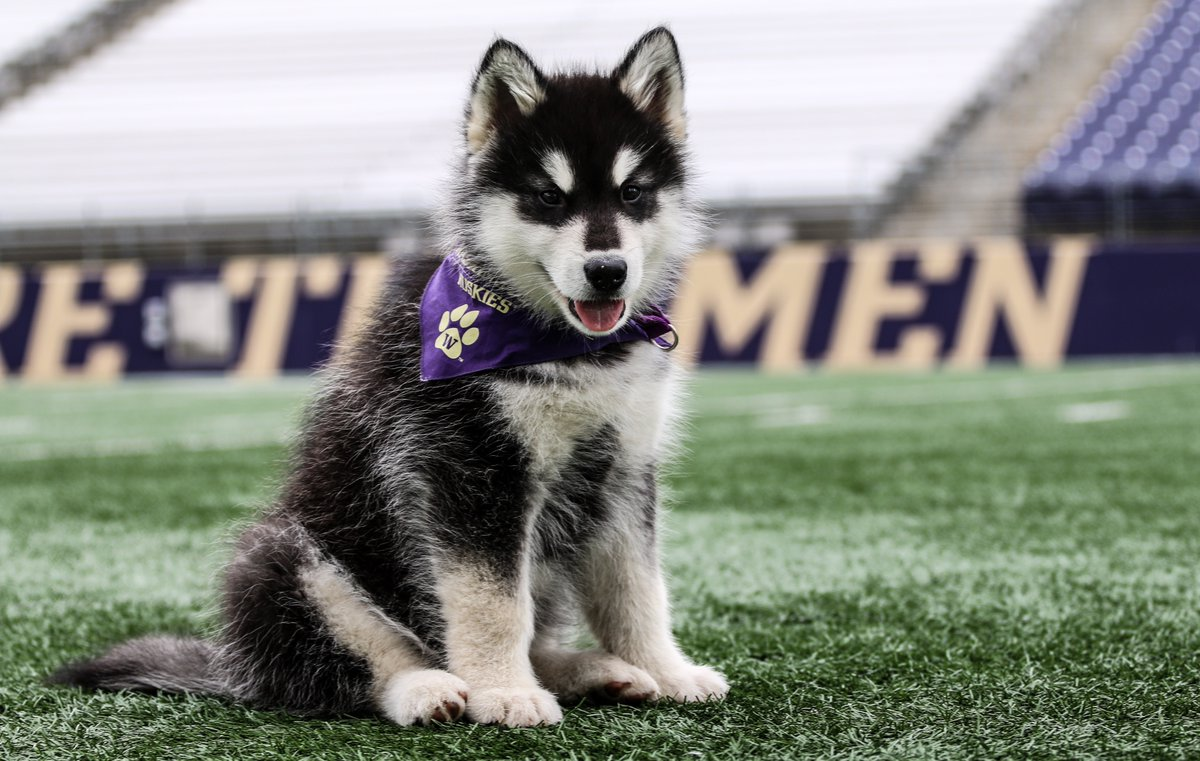
\includegraphics[width=0.5\linewidth]{dubs.jpg}
    \caption{Here is a picture of Dubs \cite{webeck_2018}. Dubs did not swallow a marble.}
    \label{fig:dubs}
\end{figure}

% Summary and Conclusions
\section{Summary and Conclusions}
Add your summary and conclusions here.

% References
\printbibliography

% Appendices
\begin{appendices}

% MATLAB Functions
\section{MATLAB Functions}
Add your important MATLAB functions here with a brief implementation explanation. This is how to make an \textbf{unordered} list:
\begin{itemize}
    \item \texttt{y = linspace(x1,x2,n)} returns a row vector of \texttt{n} evenly spaced points between \texttt{x1} and \texttt{x2}. 
    \item \texttt{[X,Y] = meshgrid(x,y)} returns 2-D grid coordinates based on the coordinates contained in the vectors \texttt{x} and \texttt{y}. \text{X} is a matrix where each row is a copy of \texttt{x}, and \texttt{Y} is a matrix where each column is a copy of \texttt{y}. The grid represented by the coordinates \texttt{X} and \texttt{Y} has \texttt{length(y)} rows and \texttt{length(x)} columns.  
\end{itemize}

% MATLAB Codes
\section{MATLAB Code}
Add your MATLAB code here. This section will not be included in your page limit of six pages.

\begin{listing}[h]
\inputminted{matlab}{example.m}
\caption{Example code from external file.}
\label{listing:examplecode}
\end{listing}

\end{appendices}

\end{document}
